\documentclass[12pt,a4paper,titlepage]{article}
\usepackage[utf8]{inputenc}
\usepackage[finnish]{babel}
\usepackage{setspace}
\usepackage{parskip}
\usepackage{amssymb}
\usepackage{amsmath}
\usepackage{graphicx}
\usepackage{fancyhdr}
\usepackage[top=1in, bottom=1in, left=1in, right=1in]{geometry}
\usepackage{float}
\usepackage{ wasysym }
\usepackage{epsf} 

% hyödyllisiä paketteja:
\usepackage{siunitx}\sisetup{per=frac} % SI-yksiköitä.
%\usepackage{supertabular} % jos tarttee isoja taulukoita
%\usepackage{fullpage} % pienemmät marginaalit jos haluaa

\usepackage{hyperref} % lisääthän omat pakettisi ENNEN hyperref'iä
\hypersetup{pdfborder={0 0 0}}
\onehalfspacing
\cfoot{}
\rhead{\thepage}
% asettaa nyk. kappaleen nimen vasempaan ylänurkkaan, saa poistaa jos haluaa
\lhead{\leftmark}

% pythonjutut
\usepackage{color}
\usepackage{listings}
\usepackage{setspace}

\definecolor{Code}{rgb}{0,0,0}
\definecolor{Decorators}{rgb}{0.5,0.5,0.5}
\definecolor{Numbers}{rgb}{0.5,0,0}
\definecolor{MatchingBrackets}{rgb}{0.25,0.5,0.5}
\definecolor{Keywords}{rgb}{0,0,1}
\definecolor{self}{rgb}{0,0,0}
\definecolor{Strings}{rgb}{0,0.63,0}
\definecolor{Comments}{rgb}{0,0.63,1}
\definecolor{Backquotes}{rgb}{0,0,0}
\definecolor{Classname}{rgb}{0,0,0}
\definecolor{FunctionName}{rgb}{0,0,0}
\definecolor{Operators}{rgb}{0,0,0}
\definecolor{Background}{rgb}{0.98,0.98,0.98}

\lstset{
  literate={ö}{{\"o}}1
           {ä}{{\"a}}1
           {ü}{{\"u}}1
}
\lstdefinestyle{python}{
numbers=left,
numberstyle=\footnotesize,
numbersep=1em,
xleftmargin=1em,
framextopmargin=2em,
framexbottommargin=2em,
showspaces=false,
showtabs=false,
showstringspaces=false,
frame=l,
tabsize=4,
% Basic
basicstyle=\ttfamily\small\setstretch{1},
backgroundcolor=\color{Background},
language=Python,
% Comments
commentstyle=\color{Comments}\slshape,
% Strings
stringstyle=\color{Strings},
morecomment=[s][\color{Strings}]{"""}{"""},
morecomment=[s][\color{Strings}]{'''}{'''},
% keywords
morekeywords={import,from,class,def,for,while,if,is,in,elif,else,not,and,
or,print,break,continue,return,True,False,None,access,as,,del,except,exec,
finally,global,import,lambda,pass,print,raise,try,assert},
keywordstyle={\color{Keywords}\bfseries},
% additional keywords
morekeywords={[2]@invariant},
keywordstyle={[2]\color{Decorators}\slshape},
emph={self},
emphstyle={\color{self}\slshape},
breaklines=true,
breakatwhitespace=true
postbreak=\raisebox{0ex}[0ex][0ex]{\ensuremath{\color{red}\hookrightarrow\space}}
}

%%%%% kansilehti %%%%%
\title{TiLa II \\ Analyzing words in a text file \vspace{0.5em}}
\author{\begin{tabular}{c}
Anni Järvenpää \\ 014338836
\end{tabular}}
\date{\today}
\begin{document}
\maketitle

\newpage
\null
\thispagestyle{empty}
\addtocounter{page}{-1}
\newpage

%%%%%%%%%%%%%%% Oleellinen sisältö alkaa%%%%%%%%%%%%%%%
\section{Johdanto}
Tavoitteena on laskea tiedostossa olevien sanojen toistokertojen määrä. Tällaisia niinkutsuttuja frekvenssilistoja käytetään paljon kielitieteessä ja erityisesti korpuslingvistiikassa. Niistä on hyötyä muun muassa tekstiä koskevien hypoteesien muodostamisessa sekä tehtyjen oletusten tarkastamisessa. Lisäksi eri teksteistä saatuja frekvenssilistoja voidaan vertailla toisiinsa. \cite{kilitiede} %TODO needs moar bullshit

\section{Menetelmät}
Sanojen laskemisessa hyödynnetään binäärihakupuuta. Puu on solmuista koostuva tietorakenne, jossa jokaiseen solmuun voidaan tallentaa tietoa ja jokaisella solmulla on 1 tai 0 vanhempaa sekä $n$ lasta missä $n \in \mathbb{N}_0$. Puu voidaan esittää suunnattuina yhtenäisinä verkkoina, joissa jokaisesta solmusta on kaari jokaiseen lapseensa. \cite{cormen}

Puussa on aina tasan yksi solmu, jolla ei ole vanhempaa ja tätä solmua kutsutaan juureksi. Solmuja, joihin ei tule kaarta mistään toisesta solmusta kutsutaan lehdiksi. Solmun korkeus on kaarien määrä pisimmällä polulla solmusta lehteen. Usein puhutaan myös puun korkeudesta, jolla tarkoitetaan puun juurisolmun korkeutta. Esimerkiksi kuvassa \ref{yleinenpuu} on esitettynä puu, jonka solmuihin on tallennettu kokonaislukuja. Puun juurisolmun arvo on 5 ja lehtisolmuissa on arvot 1, 4, -1, 12, 6, 13 ja 3 sekä korkeus 3 (kaaret $5 \rightarrow 7$, $7 \rightarrow 11$ ja $11 \rightarrow 13$ tai $11 \rightarrow 3$). \cite{cormen}

\begin{figure}
\centering
\includegraphics[width=13cm]{graphs/puu.eps}
\caption{Esimerkki puusta, johon on tallennettu kokonaislukuja.}
\label{yleinenpuu}
\end{figure}

Binäärihakupuussa jokaisella solmulla on 0, 1 tai 2 lasta ja kunkin solmun vasemmasta lapsesta lähtevässä alipuussa on vain arvoltaan solmun arvoa pienempiä arvoja ja oikeassa lapsessa lähtevässä alipuussa vain solmun arvoa suurempia arvoja. Näin etsittäessä tiettyä solmua, voidaan kunkin solmun kohdalla sulkea pois toinen solmun lapsista, jolloin joudutaan tutkimaan korkeintaan puun korkeuden verran solmuja.

\begin{figure}
\centering
\includegraphics[width=7cm]{graphs/binaaripuu.eps}
\caption{}
\label{binaaripuu}
\end{figure}

Eräs toteutus 



\section{Toteutus}


\section{Tulokset}

\section{Johtopäätökset}


%\begin{figure}
%\centering
%\includegraphics[width=10cm]{directimage.jpg}
%\caption{W. M. Keck -teleskoopin kuva planeettakunnasta HR 8799 (Ben Zuckerman [CC BY 3.0])}
%\label{directimage}
%\end{figure}


%%%%% Sisältö loppuu, lähdeluettelo %%%%%
\newpage
\bibliographystyle{plain}
\bibliography{lahteet} 
%\appendix
%\newpage
%\section{Käytetty alkuarvotiedosto} \label{alkuarvot}
%\lstinputlisting[basicstyle=\ttfamily]{hr8799.txt}
%\newpage
%\section{Simulointi- ja plottausskripti} \label{skripti}
%\lstinputlisting[basicstyle=\ttfamily,language=bash,showstringspaces=false,breaklines=true]%{skripti.txt}
%\newpage
\end{document}
